%====================================================================
% CS6007 Project: findings so far in the decentralised setting
% Decentralised Single-Index Bandits (Paper A, branch Dec-SIB)
% Same template as slides/pitch/main.tex. Update the "Next steps" and
% "Status" slides as new work lands.
%====================================================================
\documentclass[11pt]{beamer}
\usetheme{Madrid}
\usecolortheme{beaver}
\usefonttheme{professionalfonts}
\usepackage[T1]{fontenc}
\usepackage[utf8]{inputenc}
\usepackage{lmodern}
\usepackage{amsmath,amssymb,amsthm}
\usepackage{graphicx}
\usepackage{hyperref}
\usepackage{tikz}
\usetikzlibrary{arrows,positioning,shapes}
\usepackage{booktabs}
\usepackage{array}
\usepackage{pifont}

\graphicspath{{figs/}}
\setbeamertemplate{navigation symbols}{}
\setbeamerfont{footnote}{size=\tiny}
\newcommand{\yes}{\textcolor{green!45!black}{\ding{51}}}
\newcommand{\no}{\textcolor{red!70!black}{\ding{55}}}
\newcommand{\todo}{\textcolor{orange!85!black}{\ding{109}}}

\title[Decentralised Single-Index Bandits]{Decentralised Single-Index Bandits}
\subtitle{Learning an unknown reward function without a server: findings so far}
\author[Harshitha \& Nischal]{\texorpdfstring{\textbf{Presented by:}\\[0.3em]\begin{tabular}{rl}\textcolor{blue}{Harshitha (23b1071)} & Dept. of CSE\\\textcolor{blue}{Nischal (23b1024)} & Dept. of CSE\end{tabular}\\[0.8em]\textbf{Course:} CS6007: Multi-Agent Machine Learning\\[0.2em]\textbf{Instructor:} Prof.\ Avishek Ghosh}{Harshitha, Nischal}}
\institute[IIT Bombay]{IIT Bombay}
\date{\small 6 October 2026}

\addtobeamertemplate{frametitle}{}{%
\begin{tikzpicture}[remember picture,overlay]
\node[anchor=north east,xshift=0.2cm,yshift=0.4cm] at (current page.north east){
\includegraphics[height=1.1cm]{iitb_logo.png}};
\end{tikzpicture}}

\begin{document}

\usebackgroundtemplate{\tikz[remember picture,overlay]\node[opacity=0.15] at ([yshift=-2cm]current page.center){
\includegraphics[width=0.6\paperwidth]{iitb_logo.png}};}
\begin{frame}\titlepage\end{frame}
\usebackgroundtemplate{}

%====================================================================
\section{Setting}
%====================================================================
\begin{frame}{Recap: single-index bandits}
\small
\begin{block}{Model}
Each round an agent sees $K$ arms $x_{t,a}\in\mathbb{R}^d$, pulls one, and observes
\[
\boxed{y_t=f(\langle x_t,\theta_*\rangle)+\eta_t}\qquad\theta_*\text{ and }f\text{ unknown},\ f\text{ possibly non-monotone.}
\]
\end{block}
\begin{block}{ZoomSIB-UCB (Dey, Bhore \& Ghosh 2026): optimal $\tilde\Theta(T^{2/3})$}
\begin{itemize}
\item \textbf{Phase 1:} explore; estimate $\theta_*$ with the Stein estimator $\hat v=\frac1{T_0}\sum_t y_tS(x_t)\propto\theta_*$, a \emph{sample mean}.
\item \textbf{Phase 2:} project $z=x^\top\hat\theta$, cut the line into bins, run \emph{sleeping} UCB over the bins available each round. State: $(n_j,S_j)$ per bin.
\end{itemize}
\end{block}
\begin{alertblock}{Our question}
\centering $N$ agents share $\theta_*$ and $f$ but \textbf{no server}: they talk only to graph neighbours.
\end{alertblock}
\end{frame}

%====================================================================
\begin{frame}{With a server vs without a server}
\small
\begin{columns}[T]
\begin{column}{0.48\textwidth}
\centering
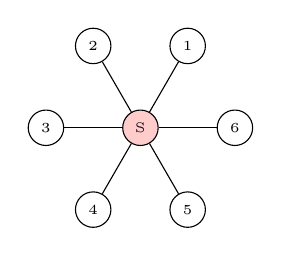
\begin{tikzpicture}[scale=0.8,every node/.style={circle,draw,minimum size=0.45cm,inner sep=0pt,font=\tiny}]
\node[fill=red!20] (s) at (0,0) {S};
\foreach \i in {1,...,6}{\node (a\i) at ({60*\i}:1.5) {\i}; \draw (s)--(a\i);}
\end{tikzpicture}\\[0.3em]
\textbf{Server (star)}\\
one coordinator sees all statistics
\end{column}
\begin{column}{0.48\textwidth}
\centering
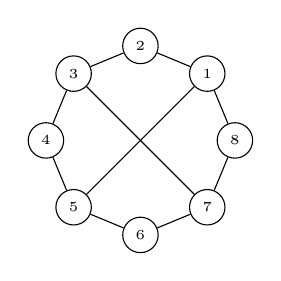
\begin{tikzpicture}[scale=0.8,every node/.style={circle,draw,minimum size=0.45cm,inner sep=0pt,font=\tiny}]
\foreach \i in {1,...,8}{\node (b\i) at ({45*\i}:1.5) {\i};}
\foreach \i/\j in {1/2,2/3,3/4,4/5,5/6,6/7,7/8,8/1,1/5,3/7}{\draw (b\i)--(b\j);}
\end{tikzpicture}\\[0.3em]
\textbf{Serverless (graph $G$)}\\
diameter $D$, spectral gap $1-\lambda$
\end{column}
\end{columns}
\vspace{0.6em}
\begin{block}{Why serverless?}
No trusted coordinator, or no backbone: sensor networks, robot/drone swarms, vehicular networks, peer-to-peer recommendation, consortia that do not share raw data.
\end{block}
\begin{center}
Network regret $R_T(N)=\sum_{i,t}\big[f(\langle x^*_{i,t},\theta_*\rangle)-f(\langle x_{i,t},\theta_*\rangle)\big]$
\end{center}
\end{frame}

%====================================================================
\begin{frame}{Our algorithm: Dec-ZoomSIB-Relay}
\small
\begin{block}{Phase 1: exact pooling without a server}
Stein sums are \textbf{sufficient statistics}: spanning-tree aggregation (up and back down a BFS tree, $2\cdot$depth rounds) gives \emph{every} agent the exact centralised $\hat\theta$.
\end{block}
\begin{block}{Freeze: one shared grid}
All agents freeze the same $\hat\theta$; the window $W$ comes from max-consensus over $D$ rounds.
\end{block}
\begin{block}{Phase 2: event-triggered flooding of bin tables}
Each agent stores the freshest copy of every agent's own $(n_j,S_j)$ table, relayed one hop per round. An agent republishes only when its unpublished count in a bin exceeds $\gamma\times$ what it currently sees.
\end{block}
\begin{alertblock}{Design principle}
\centering \textbf{Relay exact, sparse updates instead of averaging.}
\end{alertblock}
\end{frame}

%====================================================================
\section{Findings}
%====================================================================
\begin{frame}{Finding 1: collaboration pays without a server}
\small
\begin{columns}[c]
\begin{column}{0.55\textwidth}
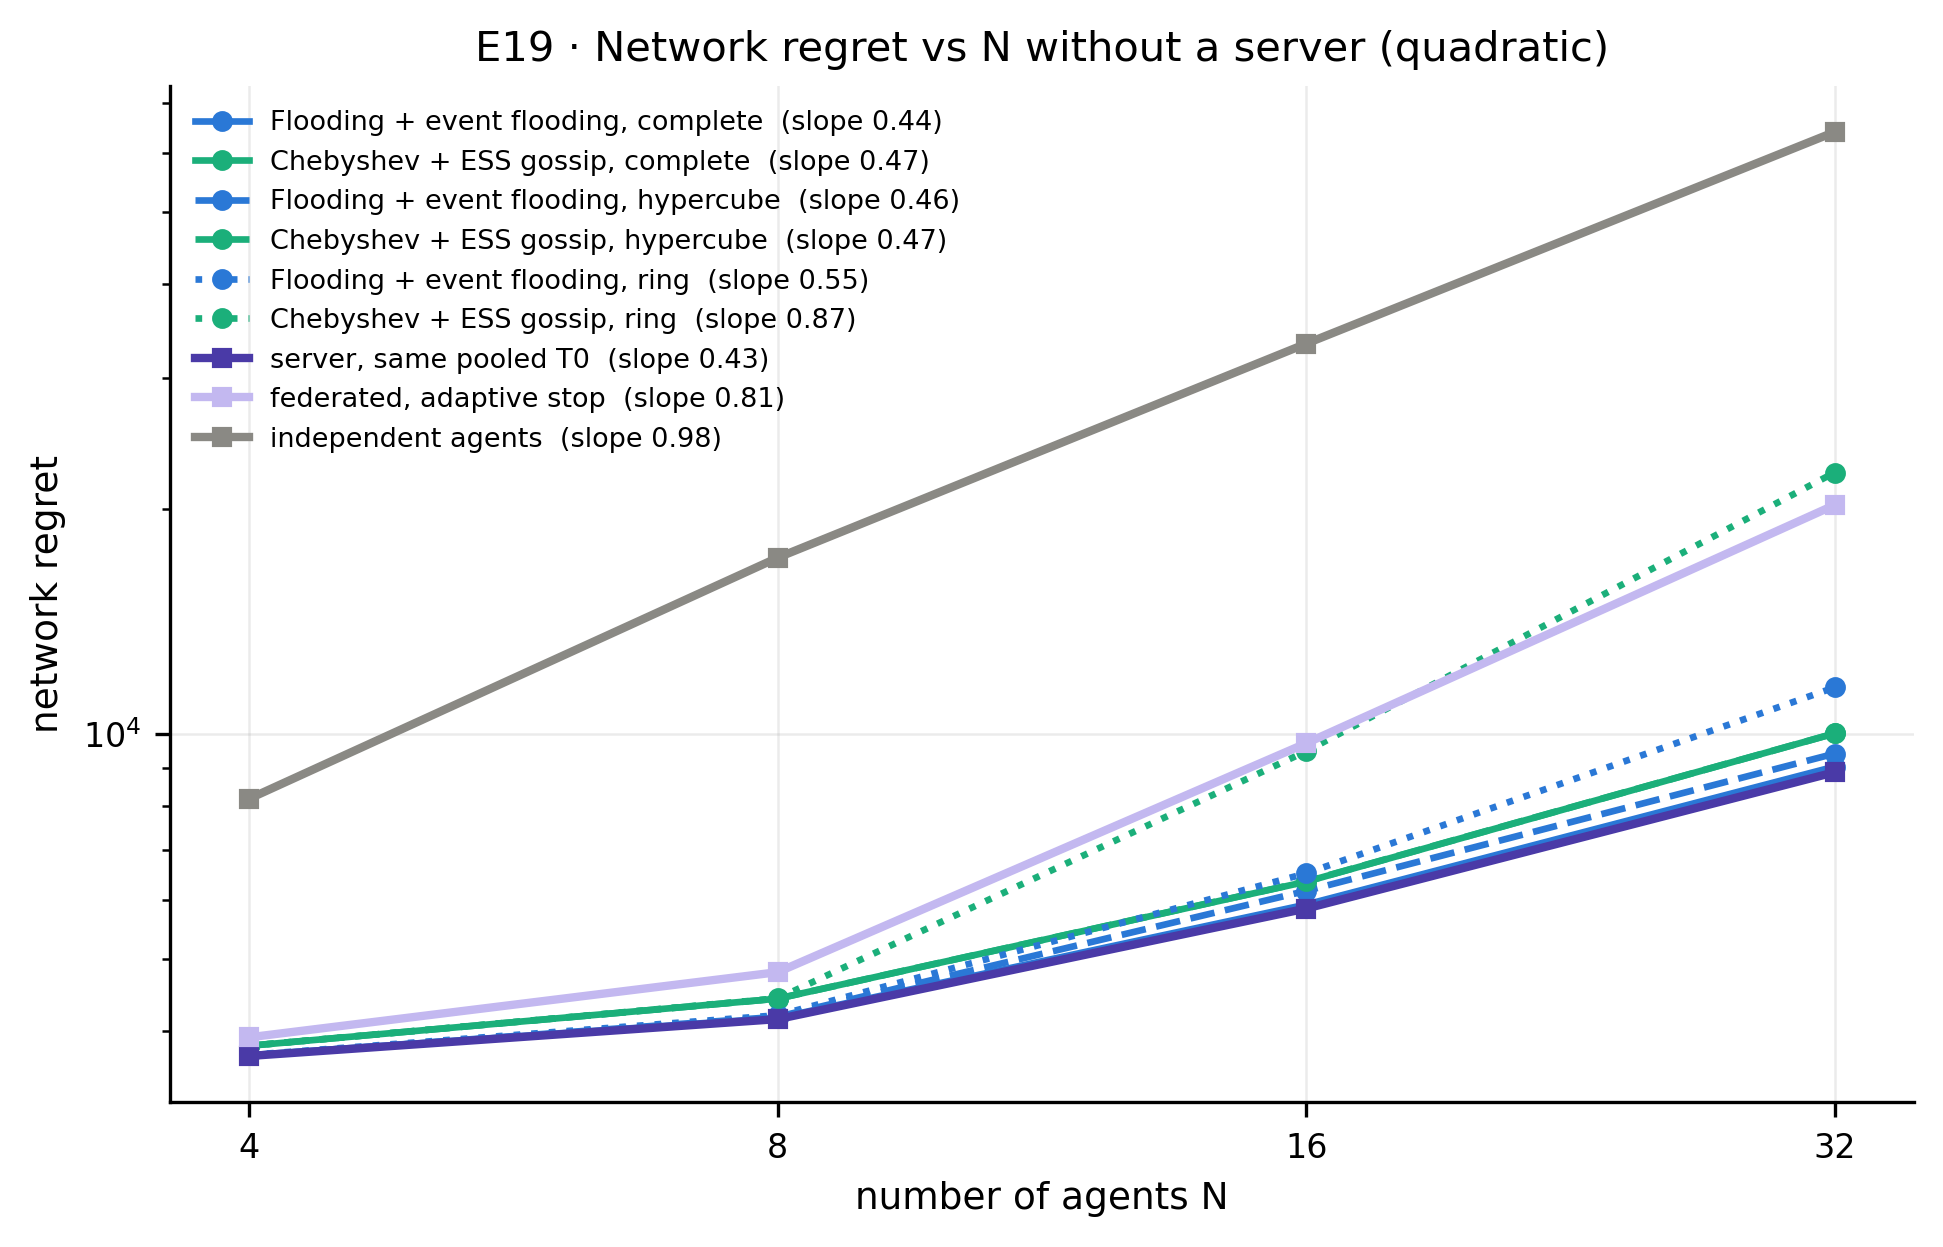
\includegraphics[width=\textwidth]{e19_scaling.png}\\
\centering\scriptsize E19, quadratic link, fixed pooled Phase-1 size
\end{column}
\begin{column}{0.43\textwidth}
Network regret $\propto N^{\alpha}$, $N=4\ldots32$:\\[0.3em]
\scriptsize
\begin{tabular}{lr}
\toprule
& $\alpha$\\
\midrule
server & 0.43\\
flooding, complete & 0.44\\
flooding, hypercube ($D=\log N$) & 0.46\\
flooding, ring ($D=N/2$) & 0.55\\
independent agents & 0.98\\
\bottomrule
\end{tabular}\\[0.5em]
\small
At $N=32$: hypercube within \textbf{6\%} of the server, ring within \textbf{30\%}.
\end{column}
\end{columns}
\end{frame}

%====================================================================
\begin{frame}{Mixing vs relaying: building a network sum}
\footnotesize
Every agent needs network totals: $\sum_i b_i$ (Phase 1) and $n_j,S_j$ per bin (Phase 2).
Toy example: ring of 4 agents with values $(4,0,0,0)$; true average $=1$.
\begin{columns}[T]
\begin{column}{0.49\textwidth}
\begin{block}{Mixing (consensus / gossip)}
Each round: $x_i\leftarrow\sum_j P_{ij}x_j$ \;(average with neighbours)\\[0.3em]
\scriptsize
\begin{tabular}{ccccc}
\toprule
round & $a_1$ & $a_2$ & $a_3$ & $a_4$\\
\midrule
0 & 4 & 0 & 0 & 0\\
1 & 1.33 & 1.33 & 0 & 1.33\\
2 & 1.33 & 0.89 & 0.89 & 0.89\\
3 & 1.04 & 1.04 & 0.89 & 1.04\\
\bottomrule
\end{tabular}\\[0.2em]
$\to1$ but \textbf{never exact}; speed set by the \emph{spectral gap}. Sends the whole state every round.
\end{block}
\end{column}
\begin{column}{0.49\textwidth}
\begin{block}{Relaying (flooding / message passing)}
Each round: forward fresher copies of \emph{each agent's own} record (with a version stamp).\\[0.3em]
\scriptsize
\begin{tabular}{cl}
\toprule
round & who knows ``$a_1$ has 4''\\
\midrule
1 & $a_2$, $a_4$\\
2 & everyone\\
\bottomrule
\end{tabular}\\[0.2em]
\textbf{Exact} after $D$ rounds (diameter); sends only records that changed.
\end{block}
\end{column}
\end{columns}
\vspace{0.1em}
\centering UCB uses counts directly ($1/\sqrt{n_j}$): mixing gives \emph{approximate} counts, relaying gives \emph{exact but stale} ones.
\end{frame}

%====================================================================
\begin{frame}{Finding 2: relaying vs mixing (E15, E18, E20)}
\scriptsize
\renewcommand{\arraystretch}{1.0}
\begin{tabular}{>{\raggedright\arraybackslash}p{4.4cm}cc}
\toprule
\textbf{Design} (torus, $N=16$, same $T_0$) & \textbf{Regret ÷ server} & \textbf{Scalars sent}\\
\midrule
Server + event-triggered sync & 1.000 & 57k\\
\alert{Spanning tree + event-triggered flooding} & \alert{1.030} & \alert{60k}\\
Flooding / consensus / push-sum every round & 1.02 & 9.5M--295M\\
\bottomrule
\end{tabular}
\vspace{0.3em}

\begin{tabular}{>{\raggedright\arraybackslash}p{4.4cm}ccc}
\toprule
\textbf{Link failures} (ratio to server) & $q=0.3$ & $q=0.6$ & $q=0.9$\\
\midrule
Flooding + event flooding & 1.06 & 1.09 & \alert{1.27}\\
Running consensus & 1.04 & 1.10 & 1.50\\
Chebyshev (accelerated) gossip & 2.1 & 3.5 & 7.3\\
\bottomrule
\end{tabular}
\vspace{0.2em}
\footnotesize
\begin{itemize}
\item \textbf{Same regret, about 2000$\times$ fewer scalars:} consensus/push-sum need 140--285M scalars.
\item On regret \emph{alone}, mixing is not worse: consensus every round is as good or slightly better on well-connected graphs (E16).
\item Relaying depends on the \emph{diameter}; mixing on the \emph{spectral gap}, and acceleration collapses when links fail.
\end{itemize}
\end{frame}

%====================================================================
\begin{frame}{When does relaying win? Scope and limitations}
\footnotesize
\begin{block}{Our claim (not ``relaying beats mixing'' in general)}
For nonparametric bandits whose sufficient statistic is a \textbf{sparse table} (bin counts and sums), relaying exact, event-triggered updates \textbf{matches the regret} of consensus-based protocols with \textbf{orders of magnitude fewer scalars}, and is more robust to sparse or unreliable graphs.
\end{block}
\begin{columns}[T]
\begin{column}{0.5\textwidth}
\begin{alertblock}{Limitations we state ourselves}
\begin{itemize}
\item Memory $O(N\cdot N_{\mathrm{bins}})$ per agent
\item Agents need unique IDs (no double counting)
\item Individual agents' statistics are shared
\end{itemize}
\end{alertblock}
\end{column}
\begin{column}{0.48\textwidth}
\begin{block}{Follow-ups that address them}
\begin{itemize}
\item \textbf{Bounded memory:} relay \emph{aggregated} tables along a spanning tree (as Phase 1 does)
\item \textbf{Privacy:} agents add noise before relaying
\end{itemize}
\end{block}
\end{column}
\end{columns}
\vspace{0.1em}
\scriptsize
\textbf{Why most papers mix:} constant memory in $N$, anonymous agents, built-in blending of data, a mature spectral-gap toolkit, and communication counted in \emph{rounds}, where both cost one message per edge.
\textbf{Precedent for relaying:} Dubey \& Pentland (Coop-KernelUCB) use message passing for the same reason: averaging biases the estimates.
\end{frame}

%====================================================================
\begin{frame}{Reference: a server $=$ one agent with $NT$ pulls}
\small
\begin{columns}[c]
\begin{column}{0.5\textwidth}
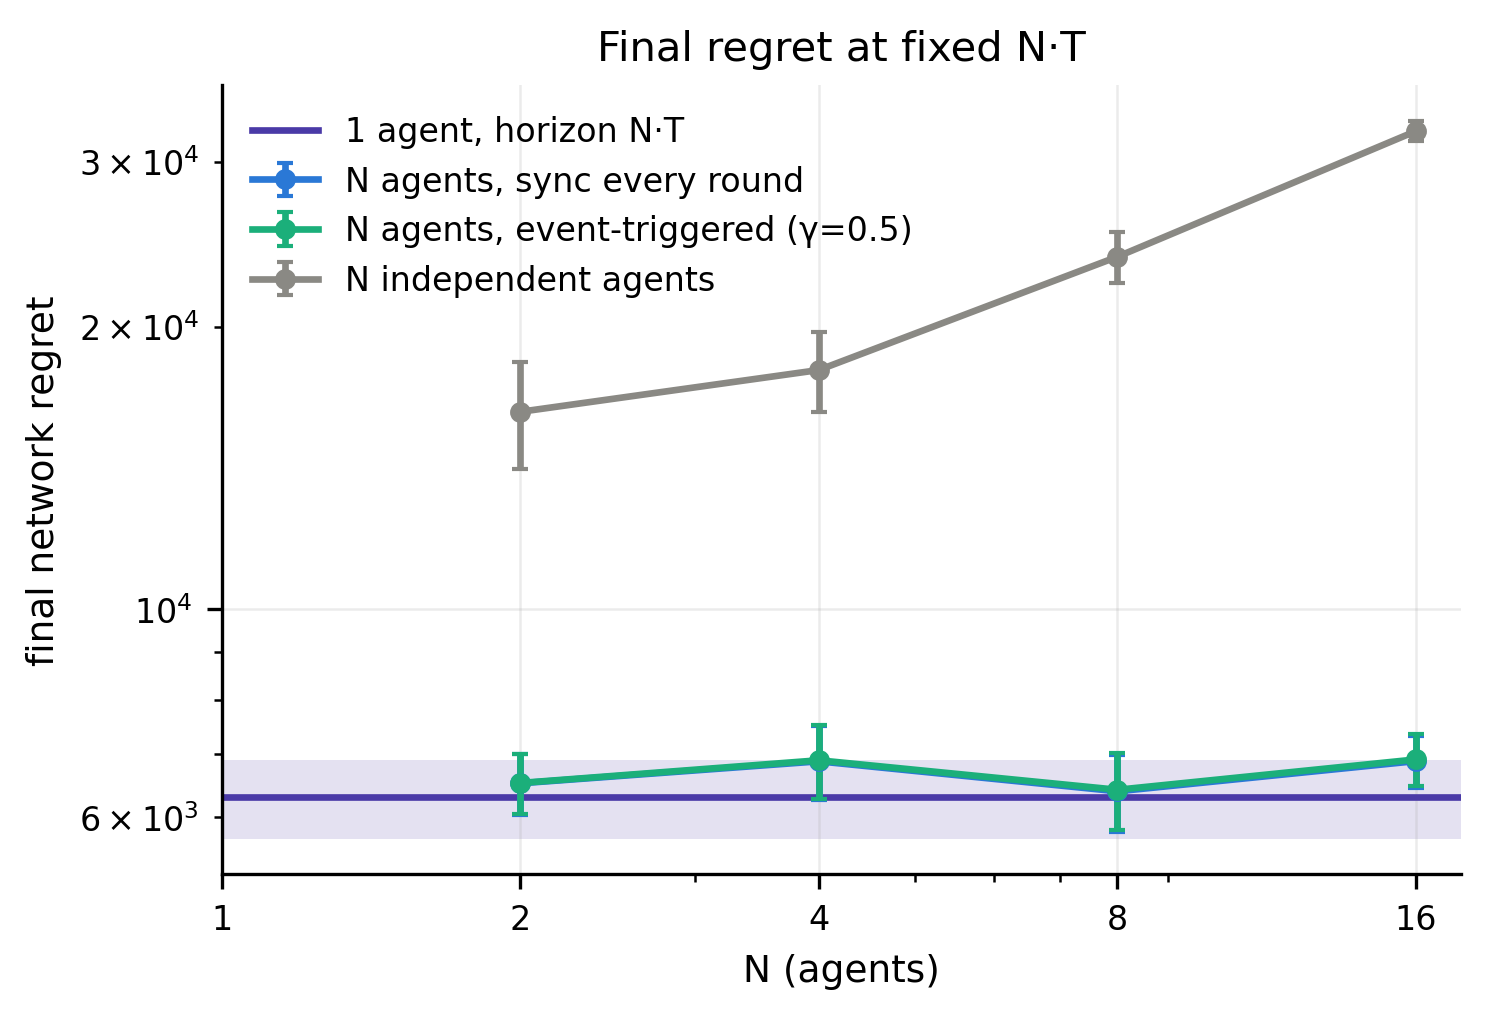
\includegraphics[width=\textwidth]{e22_vsN.png}\\
\centering\scriptsize E22: fixed budget $NT=160$k, 20 paired trials (quadratic link)
\end{column}
\begin{column}{0.48\textwidth}
\begin{itemize}
\item $N$ synced agents: within \textbf{0--10\%} of one agent at horizon $NT$, never better.
\item Independent agents: \textbf{2.3--5.1$\times$} worse.
\end{itemize}
\begin{block}{Proved (server)}
\textbf{Lower bound by simulation:} any $N$-agent algorithm $\ge c(NT)^{2/3}$.\\[0.2em]
\textbf{Upper bound:} Fed-ZoomSIB $=\tilde O\big((NT)^{2/3}\big)$.
\end{block}
\scriptsize The server rate is \emph{closed}, so it is the yardstick for the serverless version.
\end{column}
\end{columns}
\end{frame}

%====================================================================
\begin{frame}{Finding 3: what losing the server costs (E23)}
\small
\begin{columns}[c]
\begin{column}{0.5\textwidth}
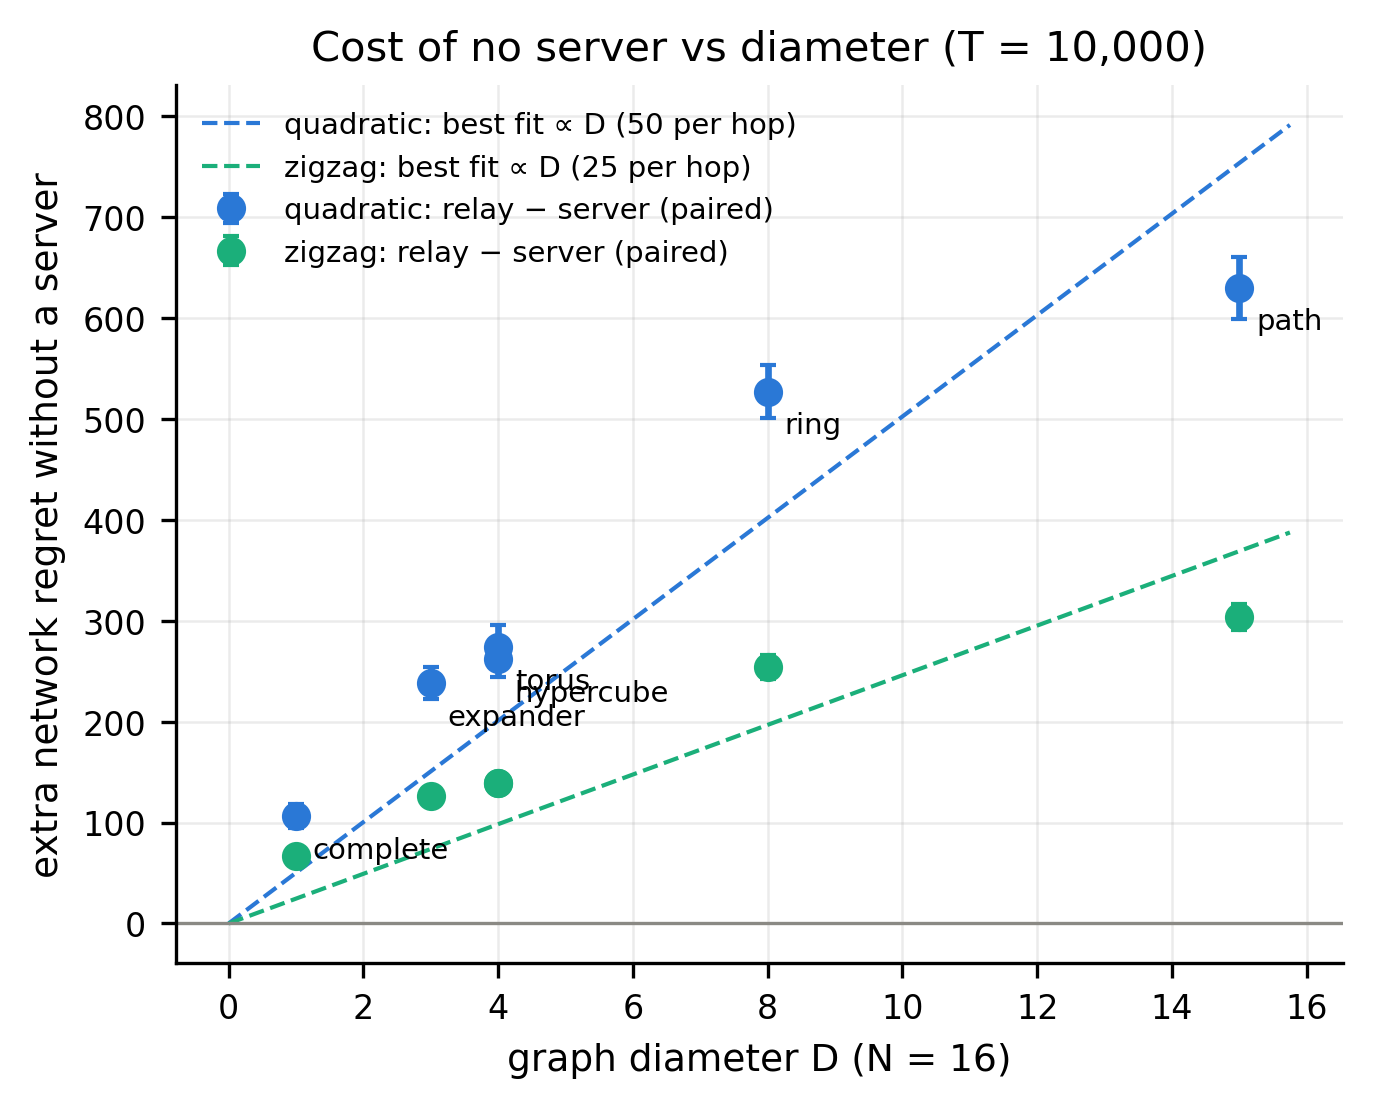
\includegraphics[width=\textwidth]{e23_vsD.png}
\end{column}
\begin{column}{0.5\textwidth}
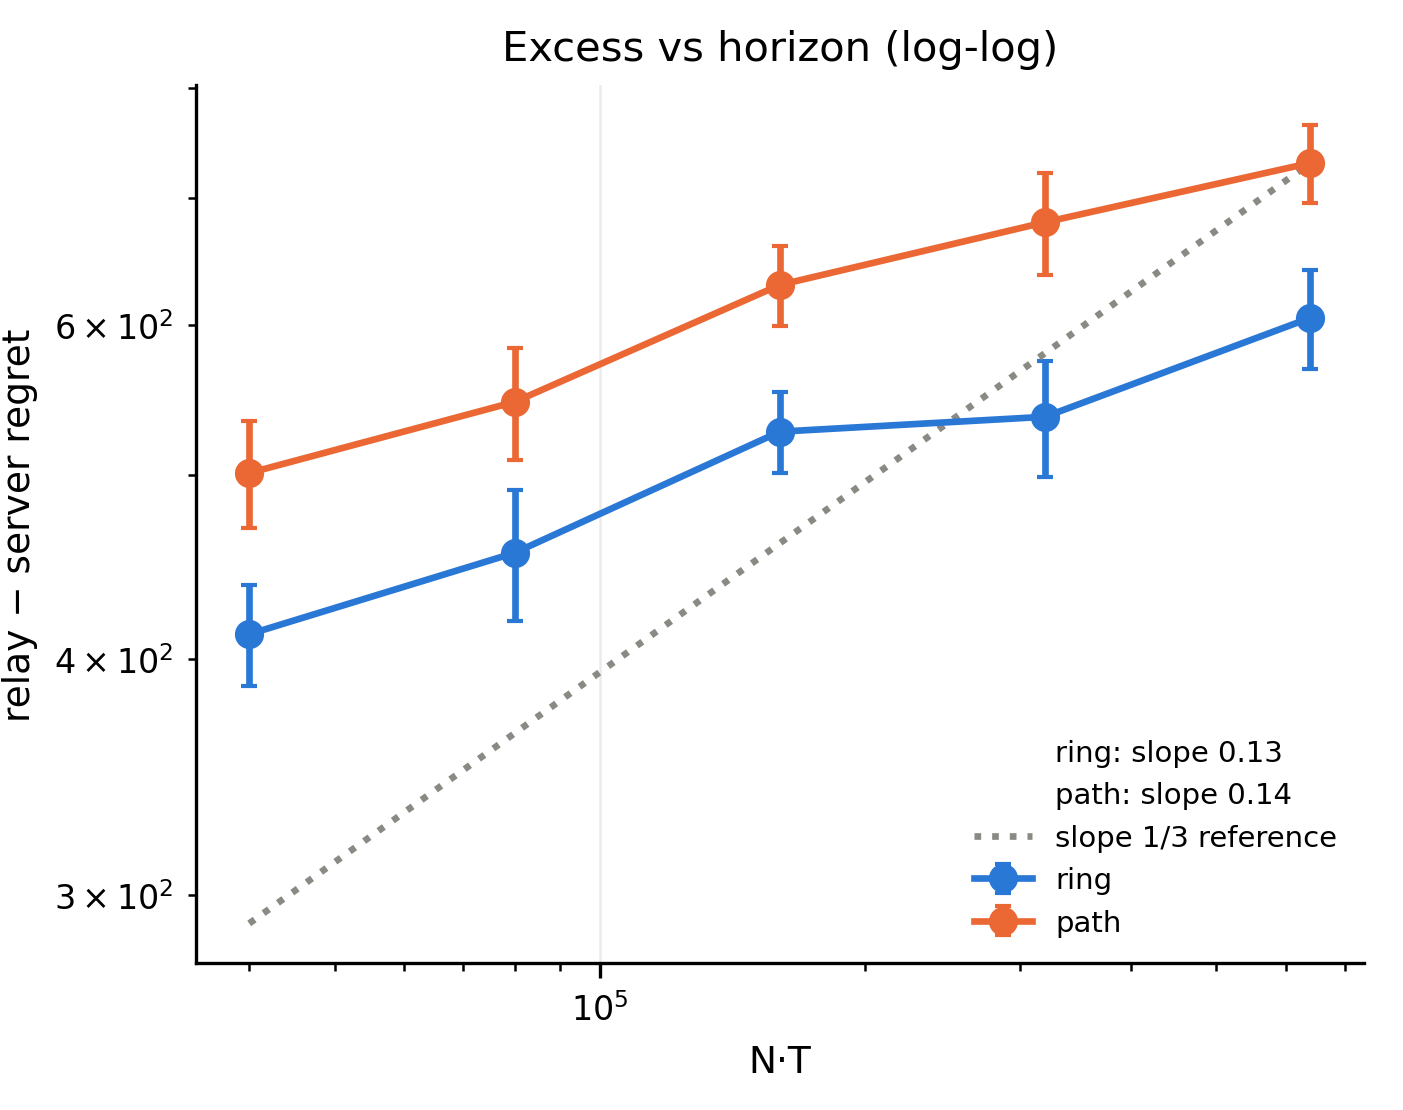
\includegraphics[width=\textwidth]{e23_vsT.png}
\end{column}
\end{columns}
\begin{itemize}
\item Extra regret: \textbf{+1.5\%} (complete, $D=1$) to \textbf{+9\%} (path, $D=15$), $N=16$; grows \emph{sublinearly} in $D$.
\item Nearly flat in the horizon: log-log slope \textbf{0.13--0.14} against the $1/3$ our bound predicts.
\item Relay sends 15--20\% \emph{fewer} scalars than the server (no broadcast to all $N$).
\end{itemize}
\end{frame}

%====================================================================
\begin{frame}{Theory: our bound vs the measurement}
\small
\begin{block}{Theorem (relay, sketch)}
\[
R_T(N)=\tilde O\big((NT)^{2/3}\big)\;+\;\underbrace{O\big(N\cdot D\cdot N_{\mathrm{bins}}\big)}_{\text{delay term}},\qquad N_{\mathrm{bins}}\sim(NT)^{1/3}
\]
\end{block}
\begin{alertblock}{The gap}
The delay term is \textbf{60--150$\times$ larger} than the measured cost, which barely grows with $T$.
\end{alertblock}
\begin{block}{Prior art says it can be tighter}
\begin{itemize}
\item DLUCB (decentralised linear): additive ``regret of delay'' only $\sim\log N/\log(1/|\lambda_2|)$.
\item Coop-KernelUCB: the graph enters as $\sqrt{\bar\chi(G)}$ (clique cover).
\end{itemize}
\end{block}
\begin{center}
\textbf{Main theory target:} only Phase-1 delay and \emph{first visits} to bins pay the diameter.
\end{center}
\end{frame}

%====================================================================
\begin{frame}{Finding 4: communication is all in Phase 2}
\small
\begin{columns}[c]
\begin{column}{0.5\textwidth}
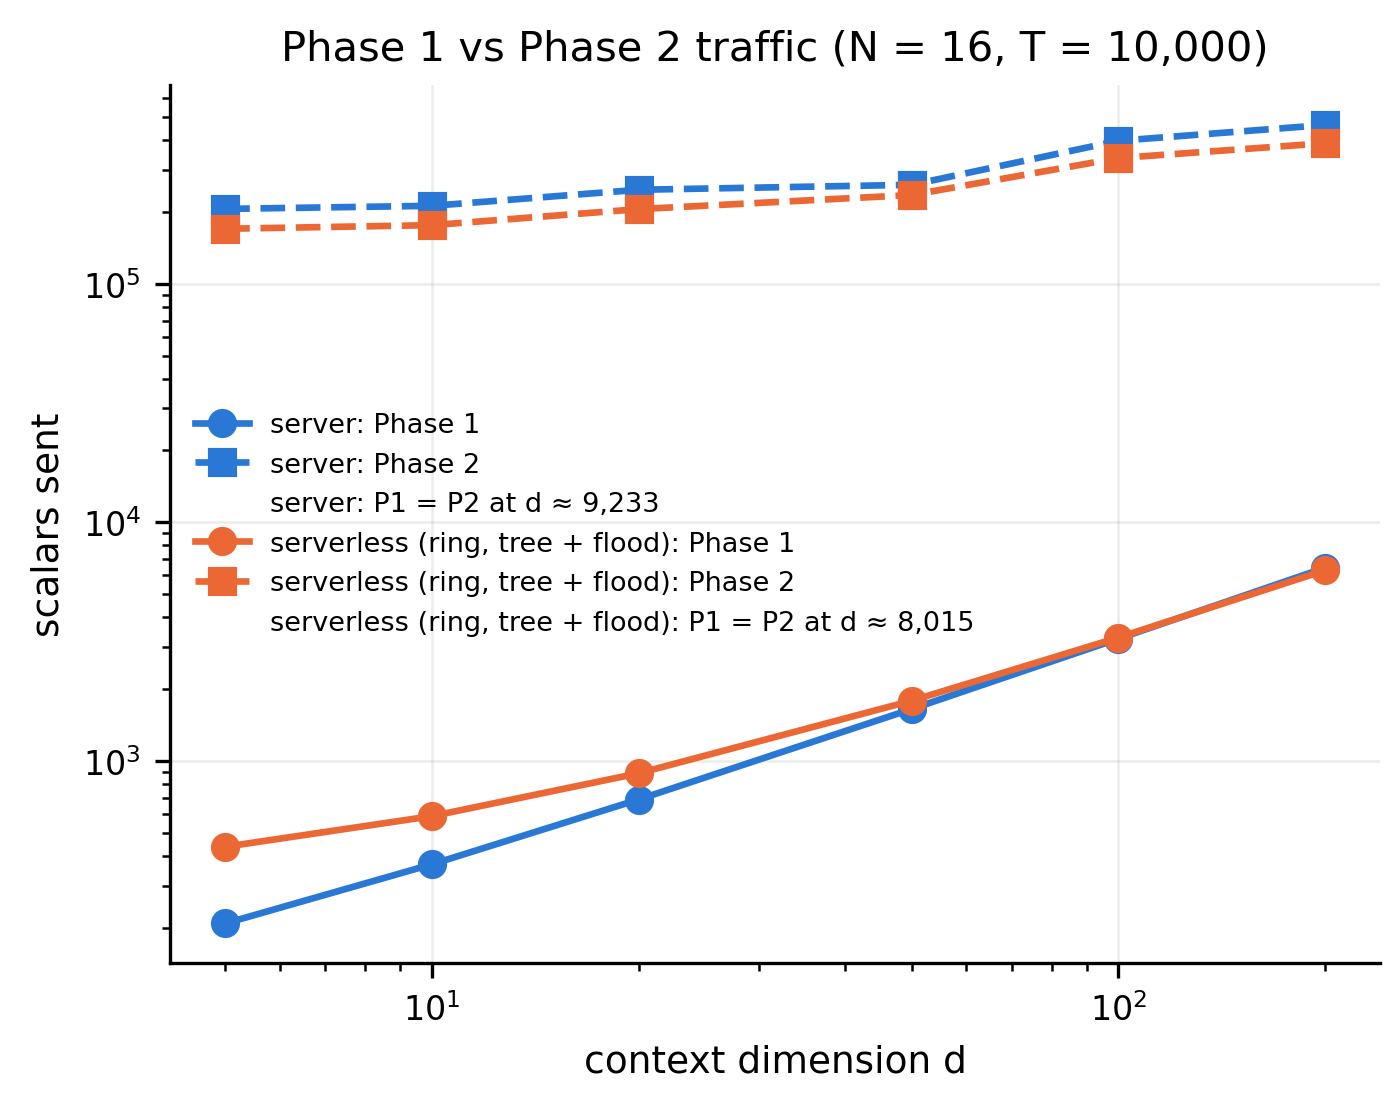
\includegraphics[width=\textwidth]{e24_traffic.png}
\end{column}
\begin{column}{0.5\textwidth}
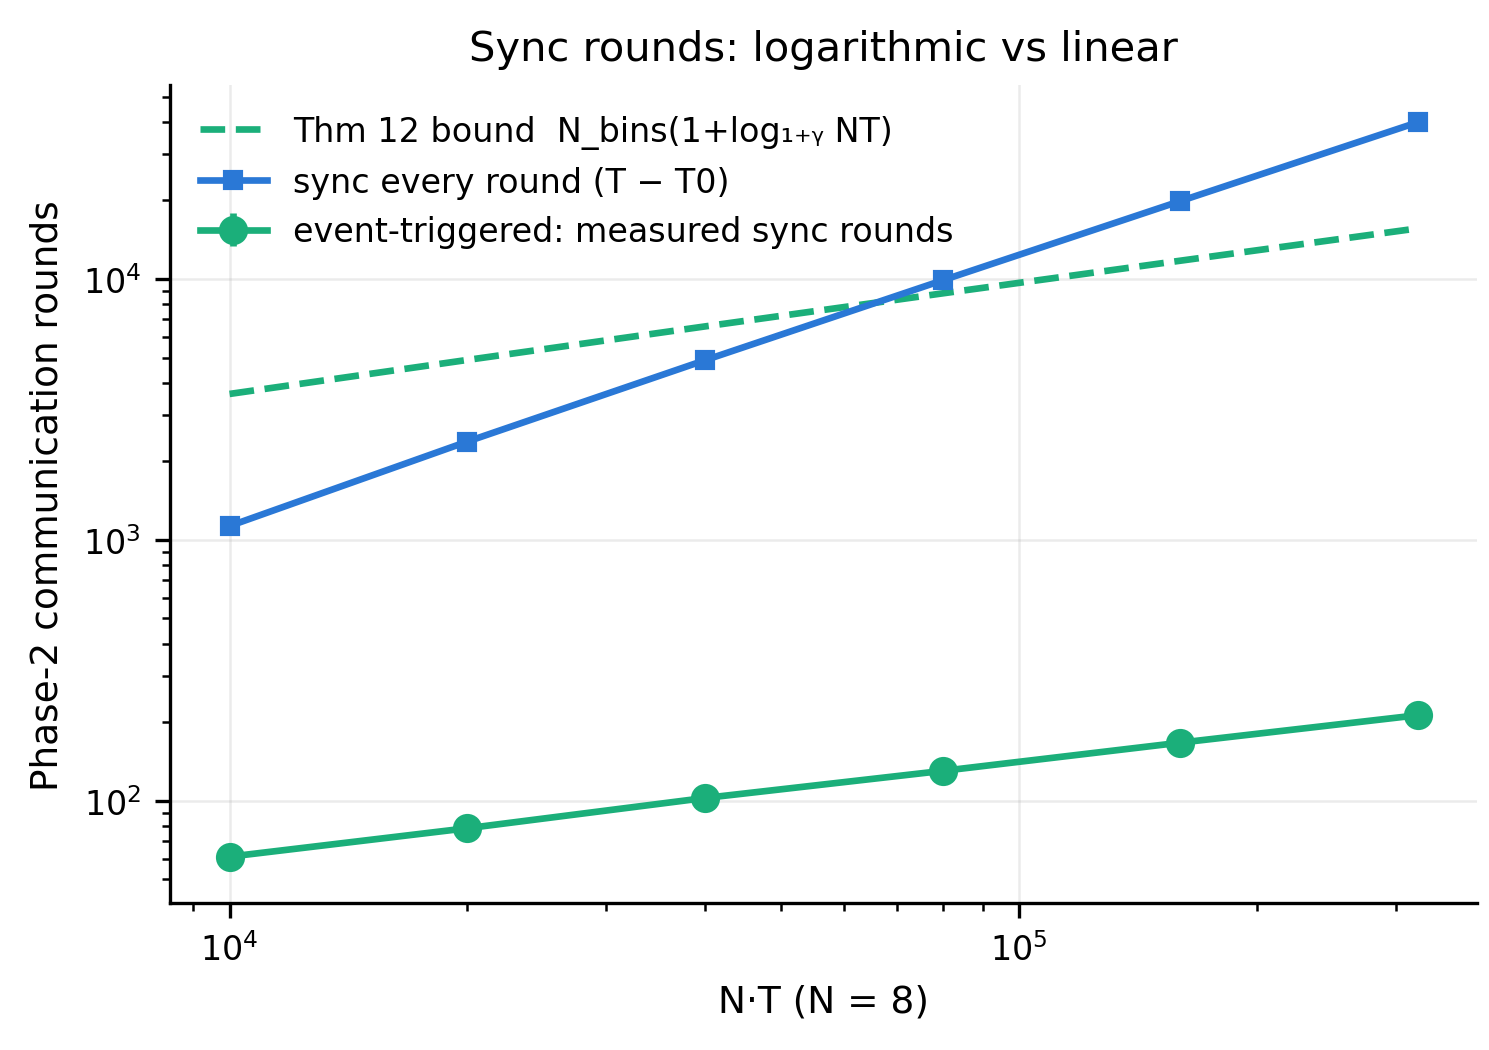
\includegraphics[width=\textwidth]{e22b_syncs.png}
\end{column}
\end{columns}
\begin{itemize}
\item Phase 1 is \textbf{0.1--1.6\%} of all traffic ($d=5\ldots200$), and shrinks with $NT$; compressing it saves $\le0.4\%$ of bits.
\item Event-triggered sync: 61$\to$213 rounds as $NT$ grows $32\times$ (per-round sync: 1k$\to$40k), at the same regret.
\end{itemize}
\end{frame}

%====================================================================
\begin{frame}{Finding 5: agents must agree, not explore longer}
\small
\begin{columns}[c]
\begin{column}{0.5\textwidth}
\centering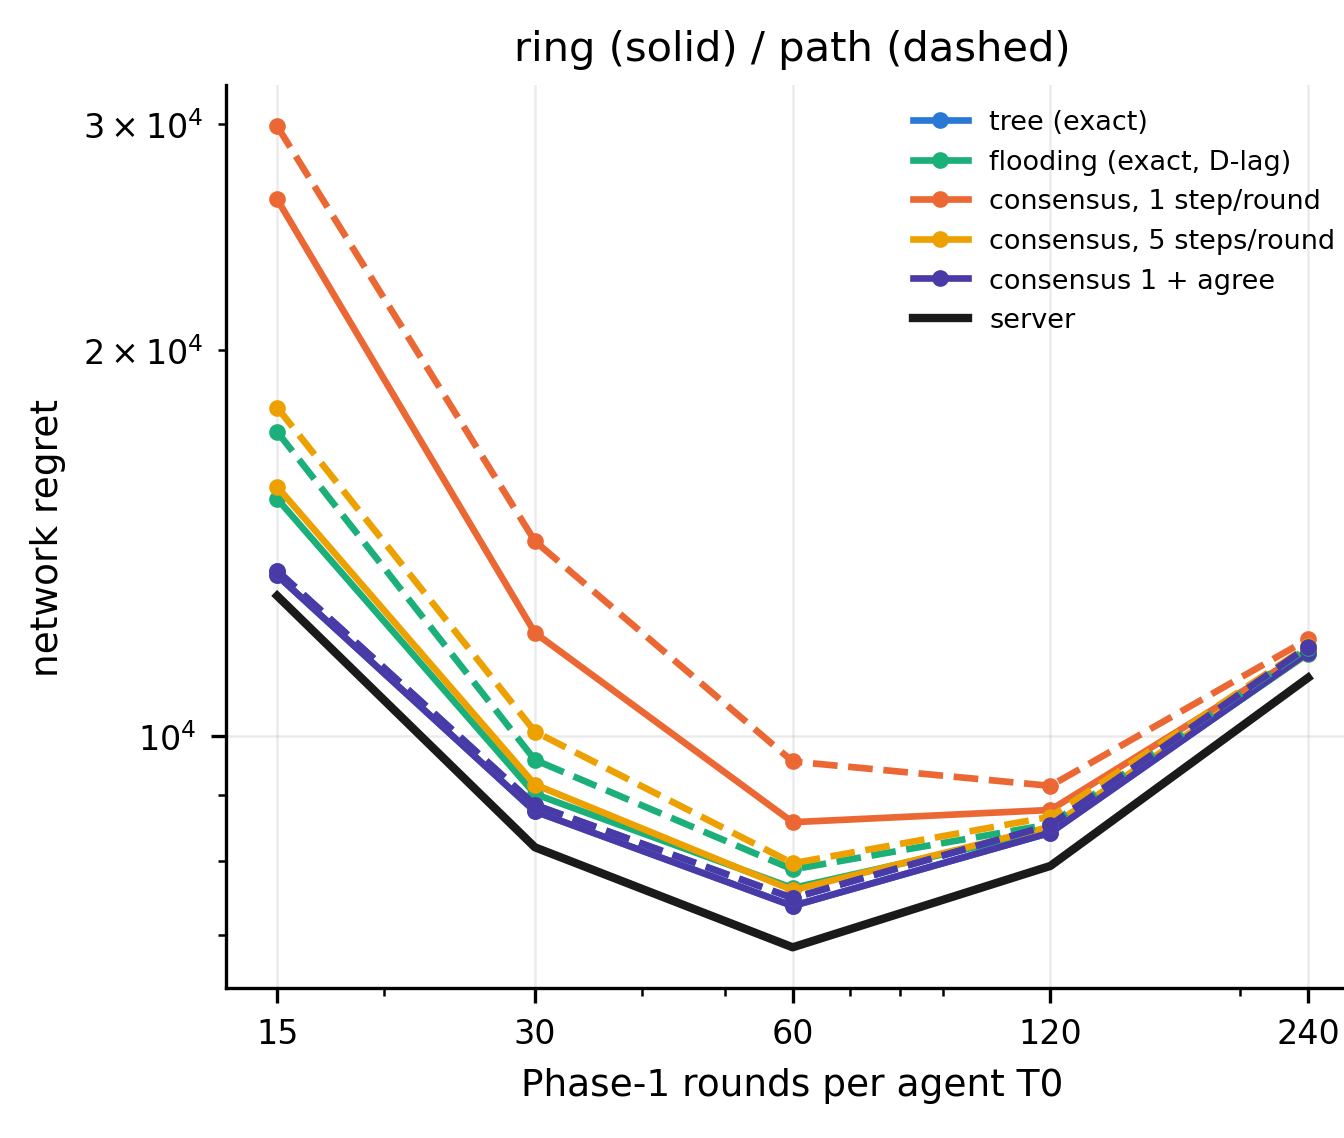
\includegraphics[width=0.9\textwidth]{e28_T0.png}
\end{column}
\begin{column}{0.5\textwidth}
\centering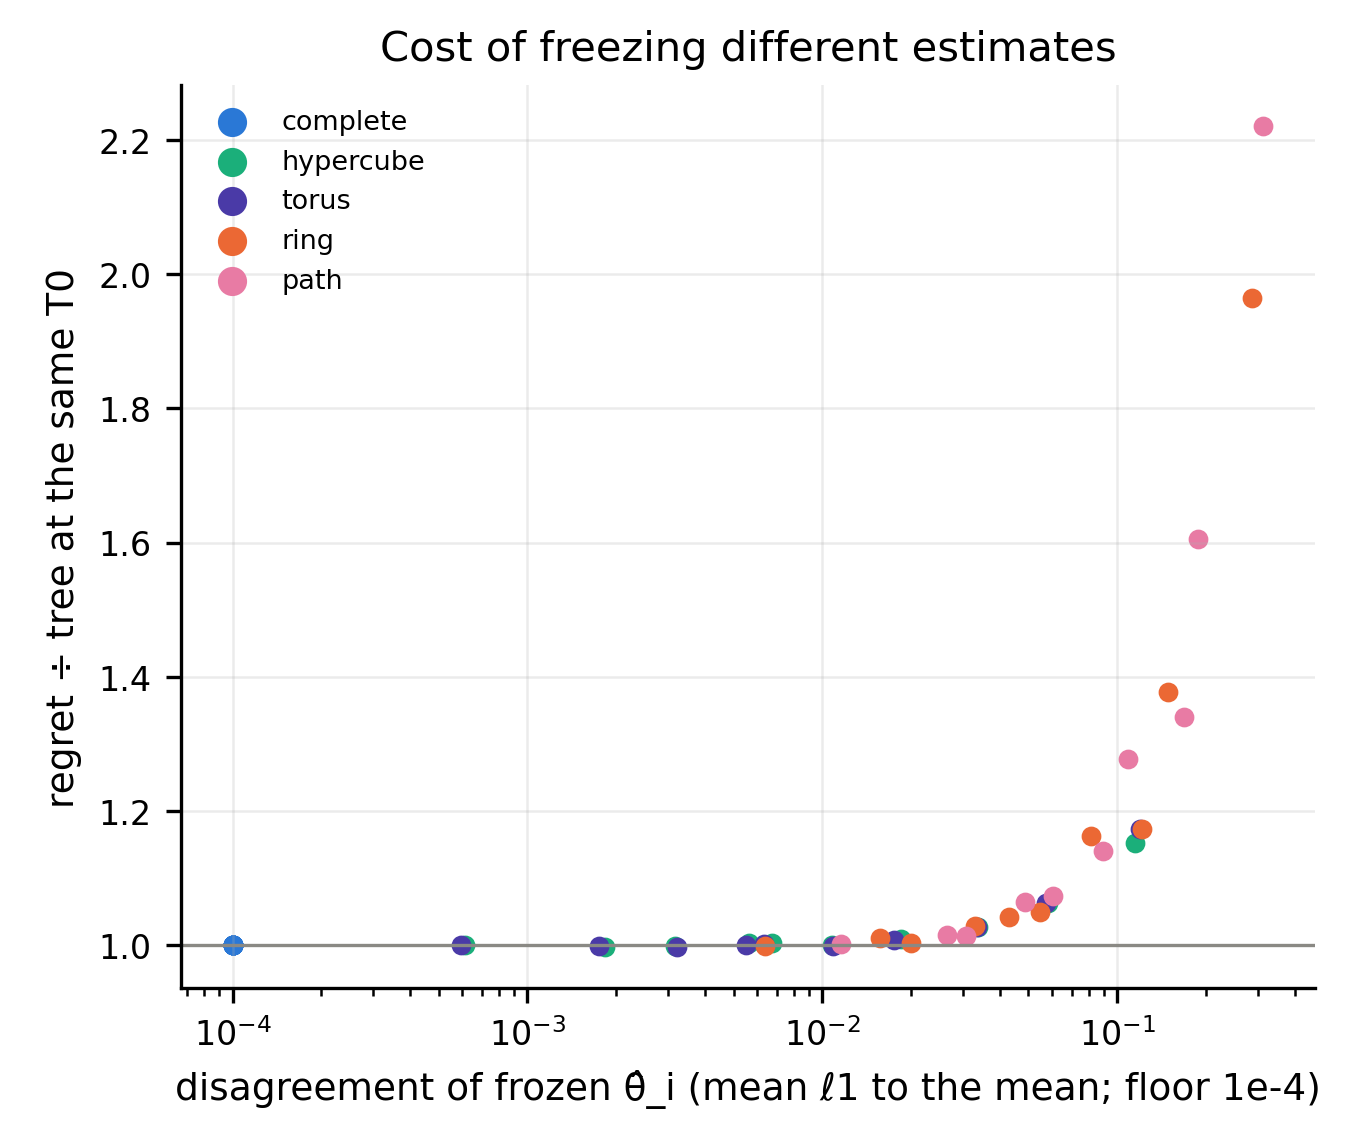
\includegraphics[width=0.9\textwidth]{e28_disagree.png}
\end{column}
\end{columns}
\begin{itemize}
\item The best exploration length $T_0^*$ barely moves with the graph.
\item The cost is agents freezing \emph{different} $\hat\theta_i$: consensus costs $\times$1.25 (ring), $\times$1.34 (path).
\item \textbf{One agreement pass} at the freeze removes it, for $\sim$2.8k extra scalars.
\end{itemize}
\end{frame}

%====================================================================
\begin{frame}{Finding 5: adaptive stopping on graphs fails}
\small
\begin{columns}[c]
\begin{column}{0.56\textwidth}
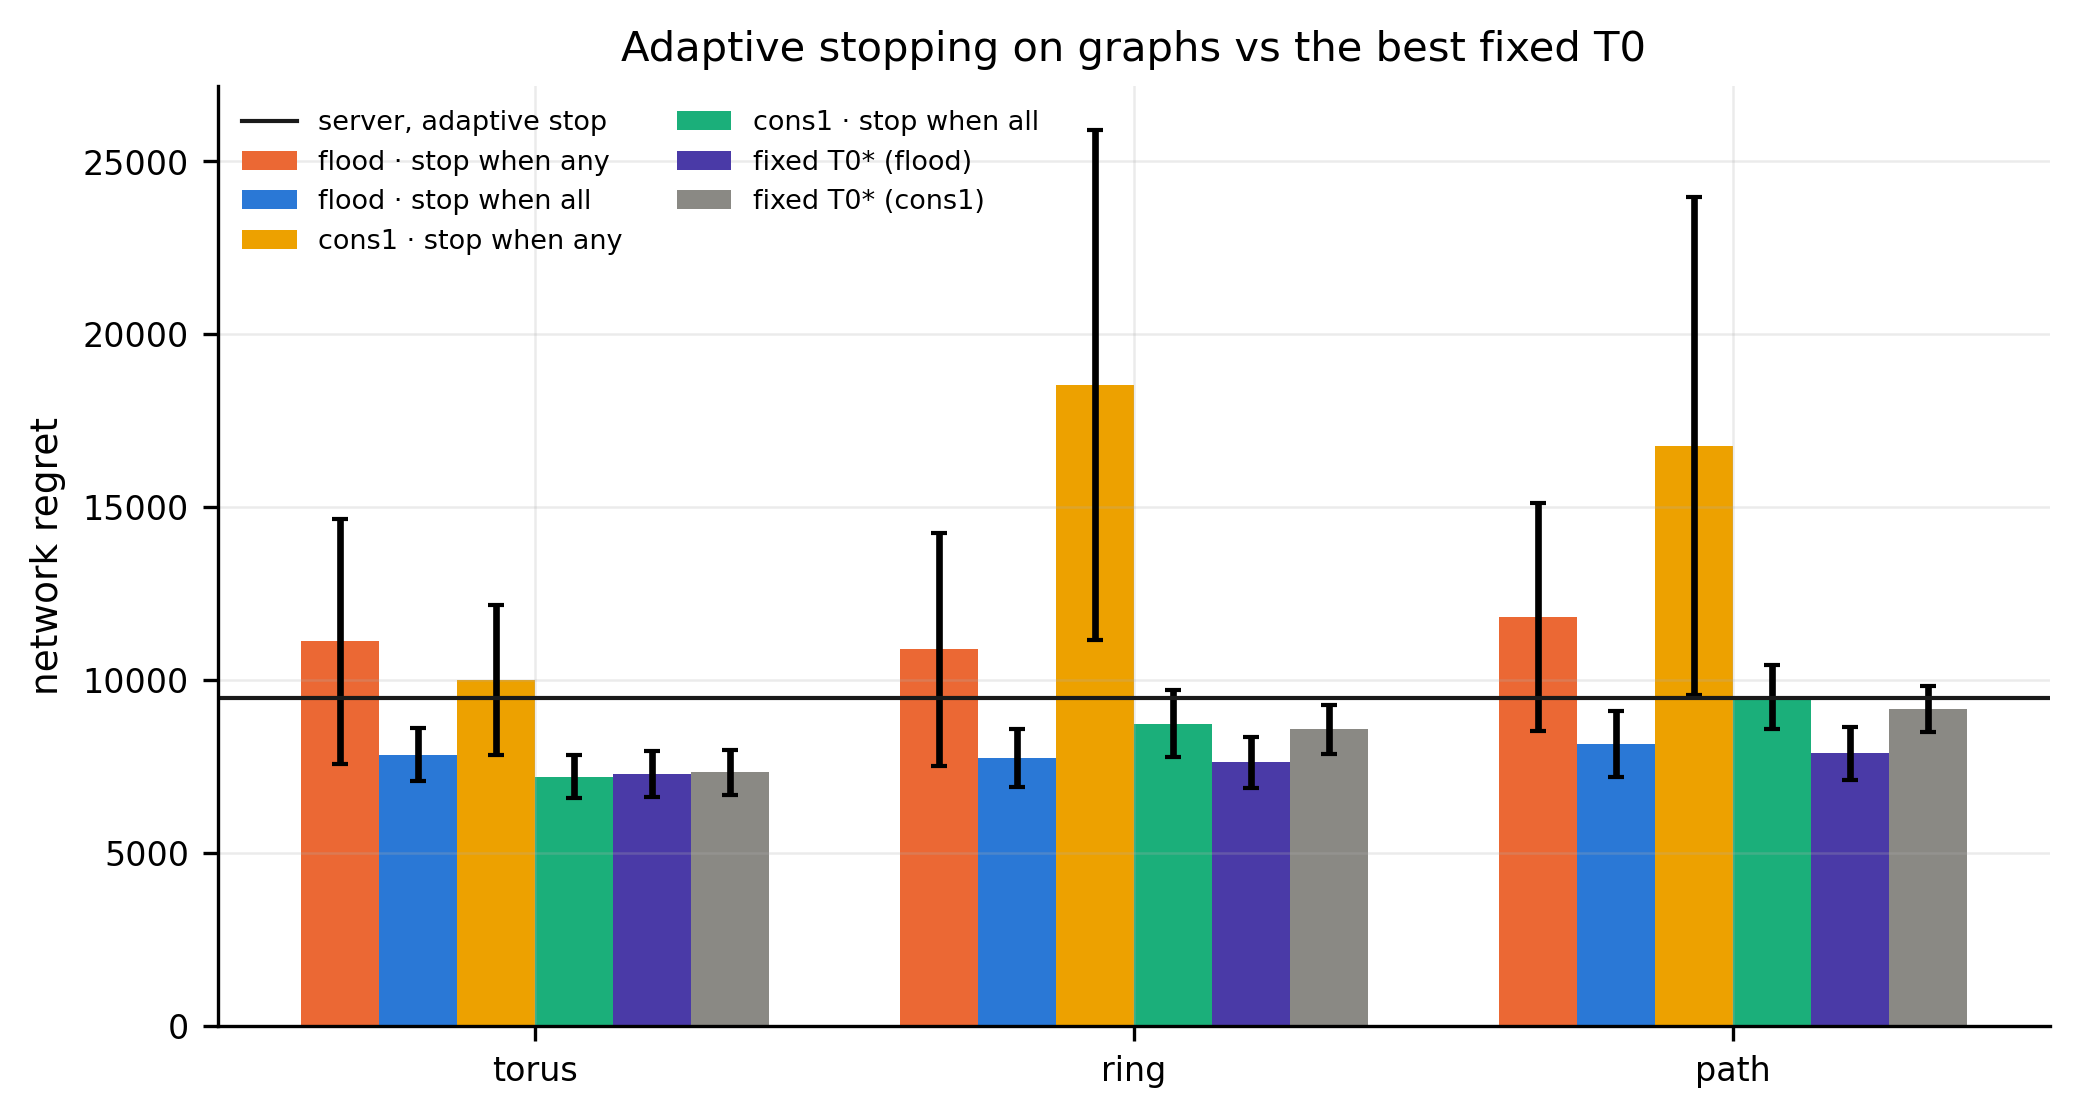
\includegraphics[width=\textwidth]{e28b_stop.png}
\end{column}
\begin{column}{0.42\textwidth}
\begin{itemize}
\item ``Stop when \emph{any} agent is stable'': \textbf{1.4--2.2$\times$} regret, high variance.
\item ``Stop when \emph{all} are'': close to fixed $T_0$, but needs $\ge D$ extra rounds to detect (not modelled).
\item Even the server's adaptive stop is worse than a fixed $T_0$.
\end{itemize}
\begin{block}{Open question}
A decentralised stopping rule that ends in \emph{agreement}, with a regret guarantee.
\end{block}
\end{column}
\end{columns}
\end{frame}

%====================================================================
\begin{frame}{Summary of findings}
\scriptsize
\renewcommand{\arraystretch}{1.2}
\begin{tabular}{>{\raggedright\arraybackslash}p{4.6cm}>{\raggedright\arraybackslash}p{5.6cm}}
\toprule
\textbf{Claim} & \textbf{Evidence}\\
\midrule
Collaboration pays without a server & regret $\propto N^{0.44\text{--}0.55}$ vs $N^{0.98}$ alone (E19)\\
Relaying: same regret, far less talk & $\times$1.03 of server at its communication; mixing needs $\sim2000\times$ more scalars (E15, E20)\\
Robust to failing links & +27\% at 90\% link failures (E18)\\
Server = one agent at $NT$ & within 0--10\%; proved lower + upper bound (E22)\\
No server costs little & +1.5\% to +9\%, nearly flat in $T$ (E23)\\
Our delay bound is loose & 60--150$\times$ above measurement (E23)\\
Communication is Phase 2 & Phase 1 $<2\%$; logarithmic sync rounds (E22, E24)\\
Agreement is what matters & disagreement $\times$1.25--1.34, fixed by one pass (E28)\\
\bottomrule
\end{tabular}
\end{frame}

%====================================================================
\section{Next}
%====================================================================
\begin{frame}{Baselines for the serverless setting}
\small
\begin{block}{1. Reference baselines (as in DLUCB, Coop-KernelUCB)}
No communication (independent ZoomSIB) \quad and \quad centralised (server) \hfill \yes\ done
\end{block}
\begin{block}{2. Prior papers' protocols, run with ZoomSIB}
Running consensus (Landgren et al.), gossip (DDUCB), accelerated consensus (DLUCB), message passing (Coop-Kernel), push-sum \hfill \yes\ done
\end{block}
\begin{block}{3. Prior papers' algorithms, run on our problems}
\begin{itemize}
\item DLUCB (decentralised linear): fails on non-monotone links \hfill \todo\ to do
\item Dec-ESTOR / Dec-GSTOR: earlier single-index methods + our communication \hfill \todo\ to do
\item Coop-KernelUCB (RBF): generic non-linear, pays in $d$ and compute \hfill \todo\ to do
\end{itemize}
\end{block}
\end{frame}

%====================================================================
\begin{frame}{Next steps (Paper A)}
\scriptsize
\renewcommand{\arraystretch}{1.0}
\begin{tabular}{>{\raggedright\arraybackslash}p{4.8cm}>{\raggedright\arraybackslash}p{3.6cm}c}
\toprule
\textbf{Work} & \textbf{Deliverable} & \textbf{Status}\\
\midrule
Server theorem: lower + upper bound & proofs (\texttt{docs/proofs}) & \yes\\
Relay theorem, full proof & Theorem with delay term & \todo\\
\alert{Tight delay term} (borrow DLUCB's technique) & additive, near-logarithmic cost & \todo\\
Lower bound in the diameter $D$ & matching necessity result & \todo\\
Agreement lemma + dec.\ stopping rule & lemma + experiment & \todo\\
Baselines: DLUCB, Dec-ESTOR/GSTOR, Coop-Kernel & experiment E29 & \todo\\
Literature check (multi-agent SIB) & related-work section & \todo\\
Bounded-memory relay; private (noisy) relay & extensions & \todo\\
Write-up & workshop / AISTATS-style draft & \todo\\
\bottomrule
\end{tabular}
\vspace{0.2em}
\begin{center}
\fbox{\parbox{0.9\textwidth}{\centering\small\textbf{Paper A:} the first single-index bandit over a network: optimal with a server, and what the graph costs without one.}}
\end{center}
\end{frame}

%====================================================================
\begin{frame}{References}
\footnotesize
\begin{enumerate}
\item D.~Dey, S.~Bhore, A.~Ghosh. \emph{Optimal Regret for Single Index Bandits.} arXiv:2605.09454, 2026.
\item Y.~Kang et al. \emph{Single Index Bandits: Generalized Linear Contextual Bandits with Unknown Reward Functions.} ICLR, 2026.
\item A.~Dubey, A.~Pentland. \emph{Kernel Methods for Cooperative Multi-Agent Contextual Bandits.} ICML, 2020.
\item S.~Amani, C.~Thrampoulidis. \emph{Decentralized Multi-Agent Linear Bandits with Safety Constraints.} AAAI, 2021.
\item D.~Mart\'inez-Rubio, V.~Kanade, P.~Rebeschini. \emph{Decentralized Cooperative Stochastic Bandits.} NeurIPS, 2019.
\item P.~Landgren, V.~Srivastava, N.~E.~Leonard. \emph{On Distributed Cooperative Decision-Making in Multiarmed Bandits.} ECC, 2016.
\item Y.~Wang, J.~Hu, X.~Chen, L.~Wang. \emph{Distributed Bandit Learning: Near-Optimal Regret with Efficient Communication.} ICLR, 2020.
\item S.~Salgia, Q.~Zhao. \emph{Distributed Linear Bandits under Communication Constraints.} arXiv:2211.02212, 2022.
\end{enumerate}
\end{frame}

%====================================================================
% thankyou.tex
% thankyou.tex

\begin{frame}[plain]
  % light colored background
  \setbeamercolor{background canvas}{bg=blue!10}
  \centering
  \vfill
  {\Huge\bfseries\color{blue!80!black} Thank You!}
  \vfill
\end{frame}
%====================================================================

\end{document}
